\documentclass[border=10pt]{standalone}
\usepackage{tikz}\usepackage{amsmath}
\usetikzlibrary{positioning, arrows.meta, calc}
\definecolor{cSrc}{HTML}{BBD9F2}\definecolor{cSelf}{HTML}{D9C7EA}
\definecolor{cAgg}{HTML}{6FA8DC}\definecolor{cTgt}{HTML}{8FCB97}\definecolor{cInk}{HTML}{222222}
\begin{document}
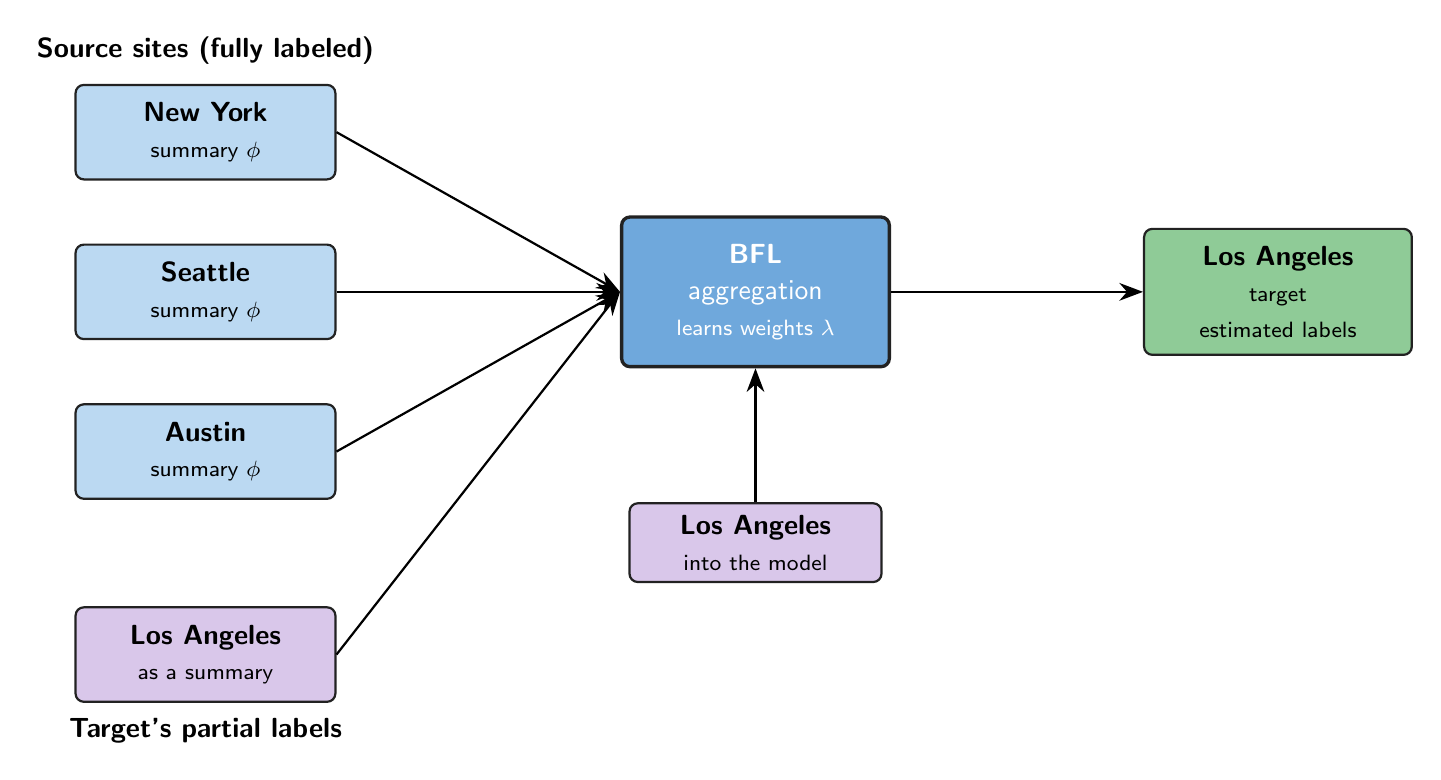
\begin{tikzpicture}[font=\sffamily,
  src/.style={draw=cInk,thick,rounded corners=3pt,fill=cSrc,align=center,minimum width=3.3cm,minimum height=1.2cm,inner sep=3pt},
  self/.style={draw=cInk,thick,rounded corners=3pt,fill=cSelf,align=center,minimum width=3.3cm,minimum height=1.2cm,inner sep=3pt},
  agg/.style={draw=cInk,very thick,rounded corners=3pt,fill=cAgg,align=center,minimum width=3.4cm,minimum height=1.9cm,text=white},
  tgt/.style={draw=cInk,thick,rounded corners=3pt,fill=cTgt,align=center,minimum width=3.4cm,minimum height=1.6cm},
  chip/.style={draw=cInk,thick,rounded corners=3pt,fill=cSelf,align=center,minimum width=3.2cm,minimum height=1.0cm,inner sep=2pt},
  arr/.style={-{Stealth[length=3mm]},thick},
  lbl/.style={font=\sffamily\small\itshape,text=cInk}]
  \node[src] (ny) {\textbf{New York}\\[1pt]\footnotesize summary $\phi$};
  \node[src, below=0.8cm of ny] (se) {\textbf{Seattle}\\[1pt]\footnotesize summary $\phi$};
  \node[src, below=0.8cm of se] (au) {\textbf{Austin}\\[1pt]\footnotesize summary $\phi$};
  \node[agg, right=3.6cm of se] (bfl) {\textbf{BFL}\\[1pt]aggregation\\[1pt]\footnotesize learns weights $\lambda$};
  \node[tgt, right=3.2cm of bfl] (la) {\textbf{Los Angeles}\\[1pt]\footnotesize target\\[1pt]\footnotesize estimated labels};
  \node[self, below=1.35cm of au] (self) {\textbf{Los Angeles}\\[1pt]\footnotesize as a summary};
  \node[chip, below=1.7cm of bfl] (lab) {\textbf{Los Angeles}\\[1pt]\footnotesize into the model};
  \draw[arr] (ny.east) -- (bfl.west); \draw[arr] (se.east) -- (bfl.west); \draw[arr] (au.east) -- (bfl.west); \draw[arr] (self.east) -- (bfl.west); \draw[arr] (bfl.east) -- (la.west); \draw[arr] (lab.north) -- (bfl.south);
  \node[font=\sffamily\bfseries] at ($(ny.north)+(0,0.42)$) {Source sites (fully labeled)};
  \node[font=\sffamily\bfseries] at ($(self.south)+(0,-0.35)$) {Target's partial labels};
\end{tikzpicture}
\end{document}
